% !TeX program = xelatex
\documentclass[12pt,a4paper]{ctexart}

\usepackage[top=2.5cm, bottom=2.5cm, left=2.8cm, right=2.8cm]{geometry}
\usepackage{graphicx}
\usepackage{booktabs}
\usepackage{caption}
\usepackage{hyperref}
\usepackage{amsmath}
\usepackage{array}
\usepackage{xcolor}
\usepackage{listings}

\lstset{
    basicstyle=\ttfamily\small,
    breaklines=true,
    frame=single,
    language=Python,
    numbers=left,
    numberstyle=\tiny,
    showstringspaces=false,
}

\hypersetup{
    colorlinks=true,
    linkcolor=blue,
    urlcolor=blue,
    citecolor=blue,
}

\title{本地文本文件词频统计分析}
\author{单位 \and 姓名 \and 学号}
\date{}

\begin{document}

\maketitle

\section{实验目的}

在自然语言处理领域中，词频分布分析是理解语料统计特性的基础工具。本实验选取了一个本地项目目录下的 8 个文本文件作为语料素材，这些文件以 Markdown 文档为主，夹杂 YAML 配置和 Python 脚本，构成了一份中英文混合、自然语言与代码交织的小规模文本集合。实验的出发点在于：这样的混合语料在词频统计、N-gram 分析和关键词提取中是否呈现出与纯自然语言语料不同的结构性特征，以及标准分析工具（分词器、TF-IDF、Zipf 定律检验）在这种混合语料上的适用性和局限性。

具体而言，本实验设定了三个递进的目标。第一，建立一套可同时处理中英文混合文本的分词与统计工具链，产出词频、N-gram 词组频率和 TF-IDF 关键词等多维统计量。第二，将统计结果转化为可视化图表（柱状图、直方图、词云和热力图），使分布特征可以直观地呈现和被审视。第三，通过 Zipf 定律验证（该定律预测词频与排名呈反比关系，在双对数坐标中表现为斜率接近 \(-1\) 的直线）和累积覆盖率分析，定量刻画该语料的统计特性，并结合文件间词频对比，形成对该语料内部结构与主题分布的深入认识。

\section{方法与实现}

\subsection{文本收集与预处理}

我们从目标目录递归扫描了所有文本文件，支持的扩展名包括 Markdown（\texttt{.md}）、YAML（\texttt{.yaml}、\texttt{.yml}）、Python（\texttt{.py}）和 JSON 等常用的可读文本格式。之所以选择这些格式，是因为它们在该目录下构成了全部的文件集合，且均为 UTF-8 可读的纯文本，无需额外的格式转换。扫描路径中排除了隐藏目录和输出目录，因为后者存放了分析过程中产生的 CSV 和 PNG 文件，若不排除，最终的统计将受到自身产出的循环污染。每个文件以 UTF-8 编码读取，对偶发的解码错误使用替换策略以保证流程的连续性。

\subsection{分词策略}

我们采用了双路径的分词设计。在默认路径中，我们调用 jieba 分词库对全文进行切分；jieba 能够同时识别中文词语和英文单词，对中英混合的自然语言文本有较好的适应能力，且其内置词典对常见的中文词汇覆盖较为完整。同时，我们准备了正则表达式回退路径：若 jieba 在目标环境中不可用，则退而使用正则表达式按字母和数字序列提取英文单词并统一转为小写，确保流程的鲁棒性。分词完成后，我们对结果进行停用词滤除：the、a、is、of、in 等英文高频功能词以及若干中文虚词被移除，以减少这些词对实质性内容词的统计干扰。

分流逻辑的核心代码如清单~\ref{lst:tokenize} 所示。优先路径调用 jieba 的 \texttt{lcut} 方法获得全部分词结果，然后遍历每个 token 并按语言类型分别处理：纯英文 token 转为小写，中文 token 保留原样，混合 token 则进一步拆分为子片段。

\begin{lstlisting}[caption={分词函数的分流逻辑}, label={lst:tokenize}]
def tokenize(text: str) -> List[str]:
    try:
        import jieba
        words = jieba.lcut(text)
    except ImportError:
        words = re.findall(r"[a-zA-Z0-9_]+", text.lower())
        return words
    result = []
    for w in words:
        w = w.strip()
        if not w:
            continue
        if re.fullmatch(r"[a-zA-Z0-9_]+", w):
            result.append(w.lower())
        elif re.search(r"[\u4e00-\u9fff]", w):
            w_clean = re.sub(r"[^\u4e00-\u9fff]", "", w)
            if w_clean:
                result.append(w_clean)
        else:
            sub = re.findall(r"[a-zA-Z0-9\u4e00-\u9fff]+", w)
            result.extend(s.lower() if s.isascii() else s for s in sub)
    return result
\end{lstlisting}

\subsection{统计量与分析方法}

在分词结果之上，我们计算了以下统计量。

词频：对全部 token 使用 Python 标准库 \texttt{collections.Counter} 进行计数并按频次降序排列。同时我们按文件分组计数，得到每份文档独立的词频分布，为后续的文件级对比提供了基础。单文件词频让我们能够观察每份文件的内容焦点：一份主要叙述实验流程的 Markdown 文件，其高频词与一份 Python 脚本的高频词应当呈现明显的差异。

N-gram 词组频率：我们通过滑窗方式分别提取了二元词组（bigram）和三元词组（trigram），并对各窗口的组合进行计数。整个语料被视为一个连续的 token 序列进行滑窗，因此跨句子边界的 N-gram 也会被计入。在我们的语料中，这一设计带来一个直接后果：代码片段中紧凑的 API 调用链（如 \texttt{ax.set\_title()} 被切分为 ax、set、\_、title 后，滑窗会产生 ax set、set \_ 等 bigram）在统计中获得了与自然语言搭配相近的地位。我们保留了这一设计，因为它诚实地反映了代码脚本在语料中的结构占比：代码本身就是一个密集的 token 序列，强行按句子边界截断反而会扭曲代码模式的出现频次。

TF-IDF 关键词：我们对每份文档独立计算词频（TF），并在语料层面计算逆文档频率（IDF），使用带平滑的公式 \( \text{TF} \times \log(N / (1 + \text{DF})) \)，其中 \(N\) 为文档总数，\(\text{DF}\) 为包含该词的文档数。分母中的 \(+1\) 是标准的加一平滑处理，用于避免极端情况下除零错误，同时使 IDF 值略低于未平滑版本，变体选择与实现代码一致。我们选择这一统计量的目的是识别"文件标志词"，即在某个文件中频繁出现而在全局语料中相对稀少的词汇。在一个 8 份文档的小语料中，TF-IDF 对分布极端不均匀的词格外敏感，这既是其优点（能识别文件的独有特征），也是我们后续分析中需要警觉的局限。

清单~\ref{lst:tfidf} 展示了简化 TF-IDF 的计算实现，对每份文档的词频（TF）与其逆文档频率（IDF）的乘积求和得到最终得分。

\begin{lstlisting}[caption={简化 TF-IDF 计算}, label={lst:tfidf}]
def compute_tf_idf(docs: List[List[str]]) -> Dict[str, float]:
    from math import log
    N = len(docs)
    df = Counter()
    for doc in docs:
        df.update(set(doc))
    tf_idf = {}
    for doc in docs:
        for word in set(doc):
            tf = doc.count(word) / len(doc) if doc else 0
            idf = log(N / (1 + df[word]))
            tf_idf[word] = tf_idf.get(word, 0) + tf * idf
    return tf_idf
\end{lstlisting}

Zipf 定律验证：我们将去停用词后的词频按排名降序排列，在双对数坐标系下进行线性拟合。拟合的斜率直接反映了词频分布接近幂律衰减的程度（理想的 Zipf 分布斜率为 \(-1\)）。我们不预设该语料一定服从 Zipf 定律；相反，我们将拟合结果与理论值的偏差作为分析该语料统计特性的起点。同时我们计算了累积覆盖率曲线，以量化"多少比例的高频词覆盖了语料中多少比例的总内容"；这条曲线的形状本身就能传递语料词频集中度的信息。

\subsection{可视化方案}

我们使用 matplotlib 生成全部图表，并特意将中文字体设置为文泉驿正黑（Wen\-Quan\-Yi Zen Hei）。这个选择不是可选的；若使用 matplotlib 的默认字体（DejaVu Sans），所有中文标签将显示为方框，图表将完全无法阅读。在实践中我们遇到了字体注册的问题：即使 rcParams 中声明了中文字体，matplotlib 的字体缓存也需要清除并重建才能生效；词云库（wordcloud）更是完全不读取 matplotlib 的配置，必须通过 \texttt{font\_path} 参数显式指定字体文件路径才能正确渲染中文字符。我们生成的图表统一以 180 dpi 的 PNG 格式保存，以确保在 LaTeX 编译时有足够的显示精度。

\section{实验设置}

\subsection{语料描述}

我们从目标项目目录中选取了 8 个文本文件作为语料，总字符量约 34 KB。这 8 个文件包括 1 份 YAML 配置文件、6 份 Markdown 文档和 1 份 Python 脚本。文件的内容主题围绕课程实验报告的生成流程展开：YAML 文件定义了 opencode 技能系统的注册入口；Markdown 文档（SKILL.md、README.md 以及 references/ 子目录下的四份参考文件）详细规定了实验报告生成的约束、工作流和写作规范；Python 脚本则是本次分析流水线自身的实现。语料的显著特征是中英文混合——中文承担语义叙述，英文承担变量名、函数名和代码关键词的角色。这一特征直接决定了我们分词模块的双路径设计：必须同时处理两种语言的 tokenization。

\subsection{软硬件环境}

实验的运行环境如表~\ref{tab:env} 所示。我们选择 Python 3.10 是因为 jieba（0.42.1）和 matplotlib（3.10.8）在此版本上的兼容性已在先前项目中得到验证；通过 uv 包管理器声明和锁定依赖，确保了分析脚本在任意目标机器上的可复现性，无需手动安装或版本调试。XeLaTeX 用于报告编译。受限于本地环境的字体配置，图表中文渲染经历了字体缓存清除和词云库显式字体路径指定的调试步骤；这些环境因素虽不影响统计结果本身，但对可视化产出的可读性有直接影响。

\begin{table}[htbp]
\centering
\caption{实验软硬件环境}
\label{tab:env}
\begin{tabular}{@{}lll@{}}
\toprule
类别 & 项目 & 配置 \\
\midrule
\multirow{4}{*}{硬件} & CPU & Intel Core i5-1135G7 @ 2.40GHz, 4核8线程 \\
& 内存 & 7.7 GiB \\
& 磁盘 & 1 TB SSD \\
& 架构 & x86\_64 \\
\midrule
\multirow{6}{*}{软件} & 操作系统 & Ubuntu 24.04.4 LTS \\
& Python & 3.10.13 \\
& jieba & 0.42.1 (分词) \\
& matplotlib & 3.10.8 (图表) \\
& wordcloud & 1.9+ (词云) \\
& 中文字体 & 文泉驿正黑 \\
\midrule
\multirow{2}{*}{编译} & XeLaTeX & TeX Live 2023/Debian \\
& 文档类 & ctexart \\
\bottomrule
\end{tabular}
\end{table}

\section{实验结果}

\subsection{词频分布总览}

我们对全部 8 个文件完成分词和去停用词处理后，共获得 8,882 个有效 token，去重后的唯一词数量为 1,831 个。表~\ref{tab:top10} 列出了频次最高的前十个词。

\begin{table}[htbp]
\centering
\caption{词频 Top 10}
\label{tab:top10}
\begin{tabular}{@{}rrr@{}}
\toprule
排名 & 词汇 & 频次 \\
\midrule
1 & 实验 & 87 \\
2 & ax & 64 \\
3 & 报告 & 62 \\
4 & 材料 & 47 \\
5 & 文件 & 44 \\
6 & print & 41 \\
7 & len & 41 \\
8 & 教师 & 38 \\
9 & words & 38 \\
10 & set & 38 \\
\bottomrule
\end{tabular}
\end{table}

Top10 的构成揭示了一个双语词表的结构特征。排名前三的「实验」「报告」「材料」直接对应语料的核心主题，这三个词在 SKILL.md 中作为章节标题和约束术语反复出现，其高频并非来自均匀分布，而是集中在篇幅最大的那份文件里。排在第六至第十位的 print、len、set 则是 Python 内置函数和数据类型，它们的频次（41、41、38）与中文主题词处于同一数量级。之所以 Python 关键词能达到如此高的频次，是因为分析脚本 \texttt{word\_freq\_analysis.py} 自身被纳入了统计：该脚本的 token 量为 1,721 个，占全部 token 的 19.4\%，虽然作为单一文件仅占文件数量的 1/8，但其 token 密度远高于自然语言文档。代码中的每个变量名、函数调用和符号都被分词器切分为独立的 token，而自然语言中大量的虚词和标点已被停用词过滤，这一进一出使得脚本在有效 token 统计中的权重被放大。Top30 的完整分布如图~\ref{fig:top30} 所示。

\begin{figure}[htbp]
\centering
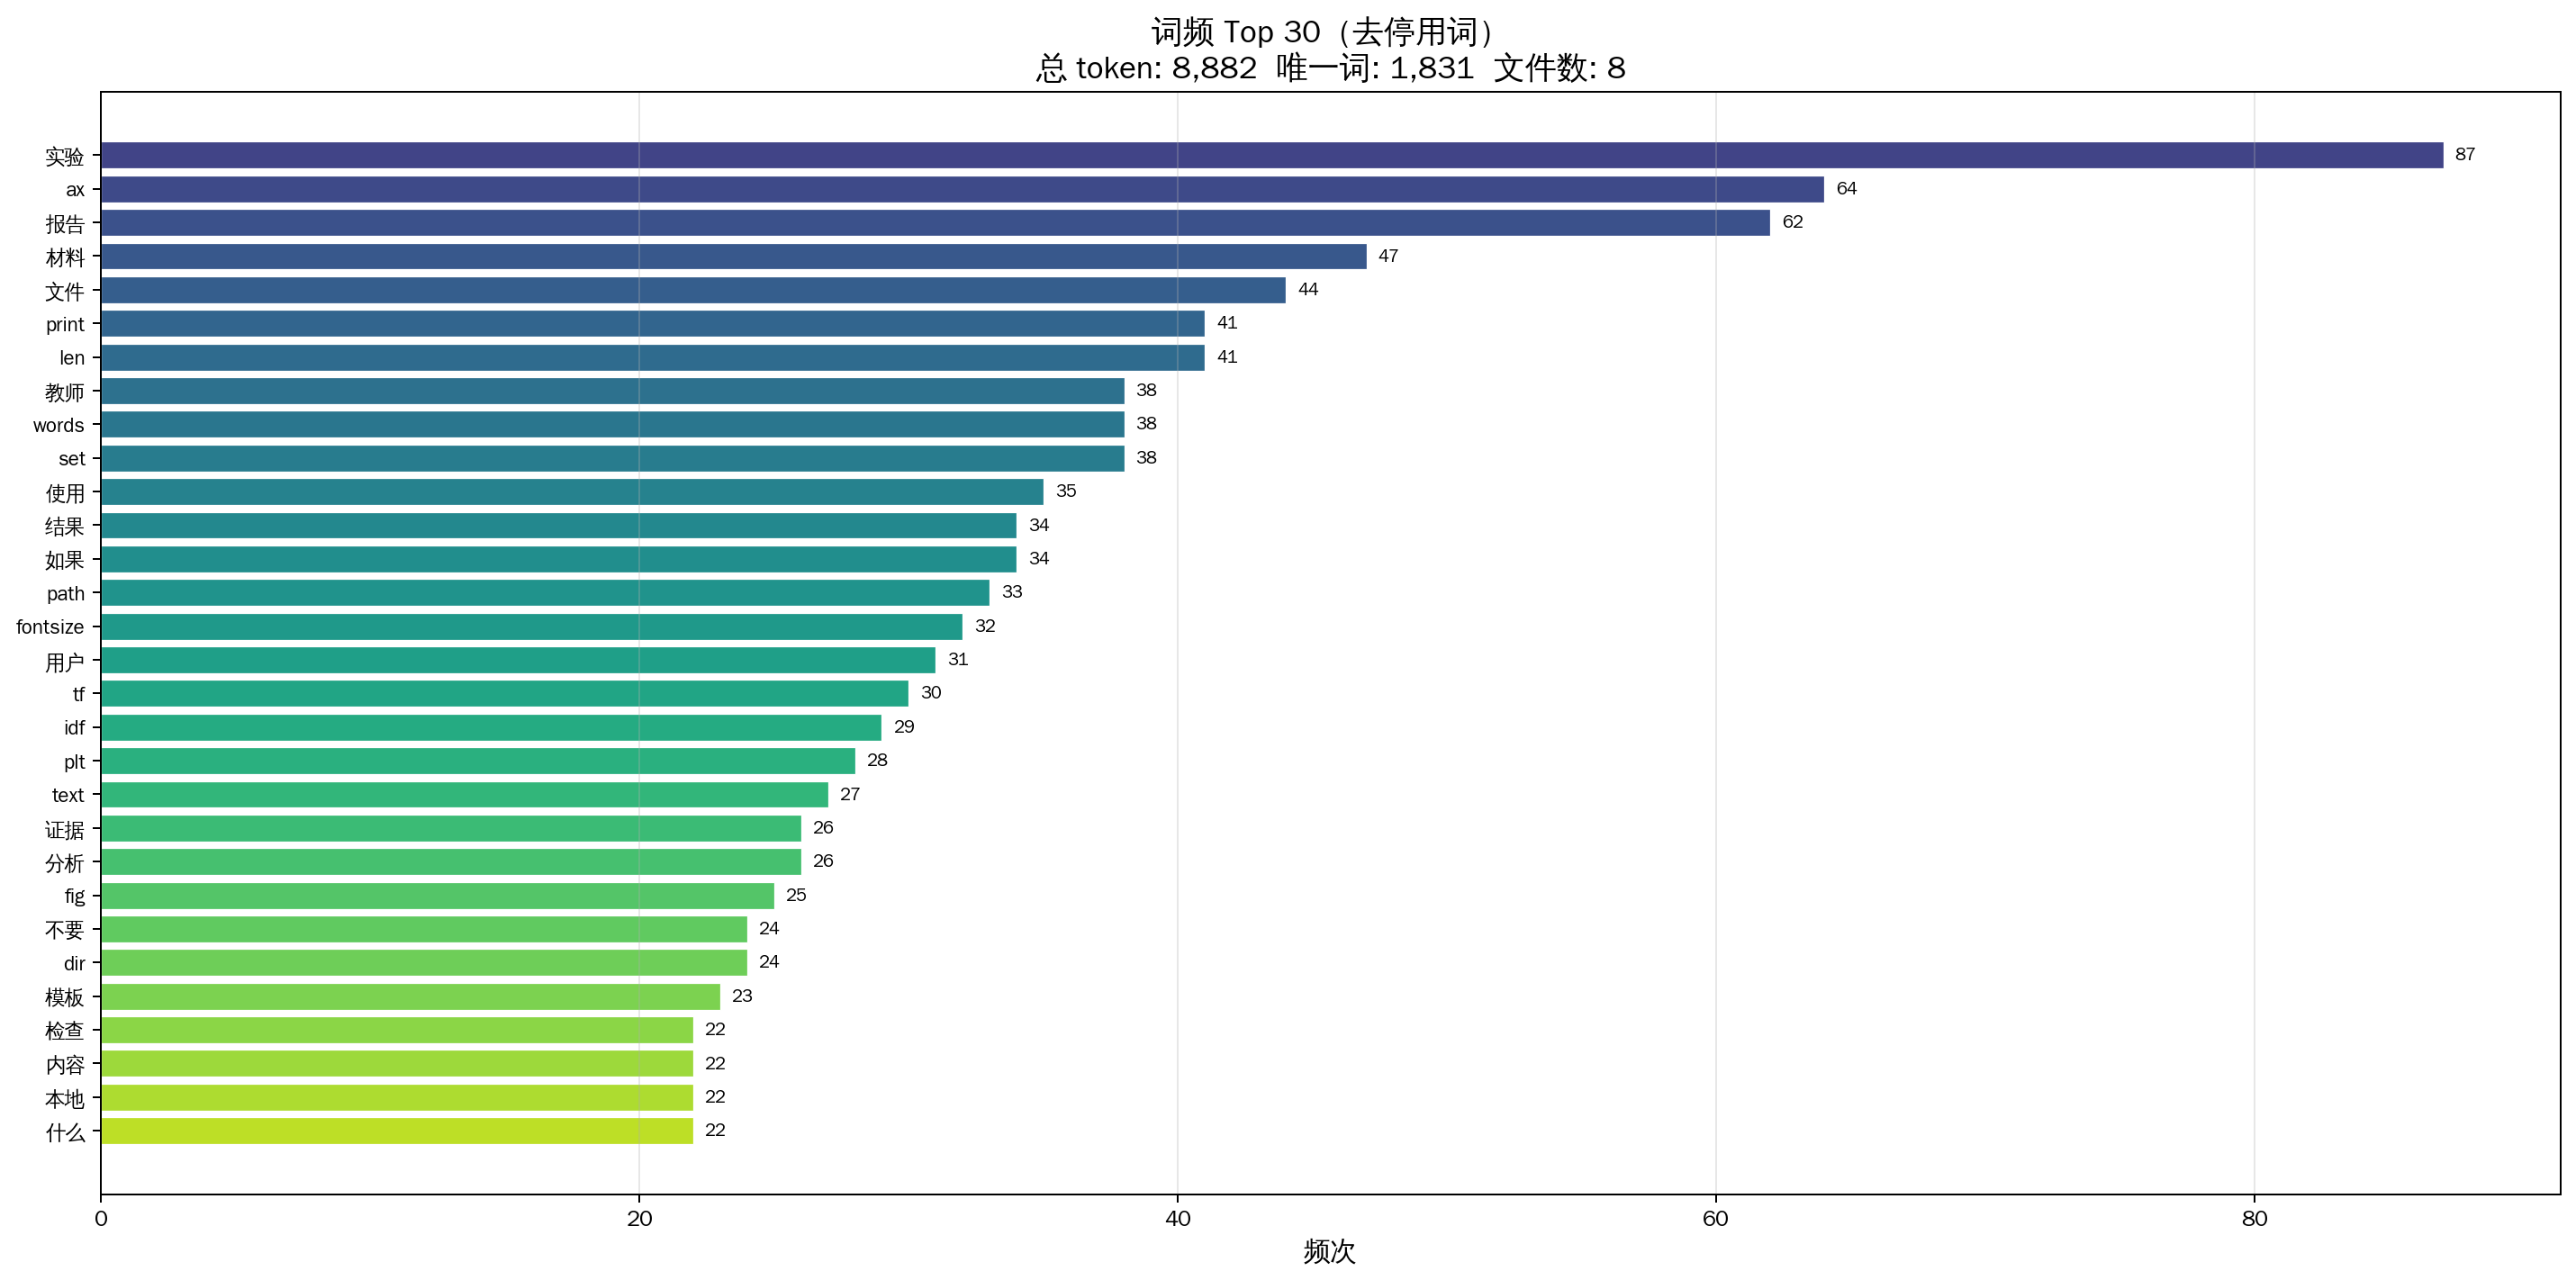
\includegraphics[width=0.92\textwidth]{figures/01_词频Top30柱状图.png}
\caption{词频 Top 30 柱状图（去停用词后）}
\label{fig:top30}
\end{figure}

\subsection{词频分布特征}

图~\ref{fig:hist} 展示了词频分布直方图——左侧为线性 Y 轴，右侧为对数 Y 轴，两个版本互补地揭示了词频的形状特征。

\begin{figure}[htbp]
\centering
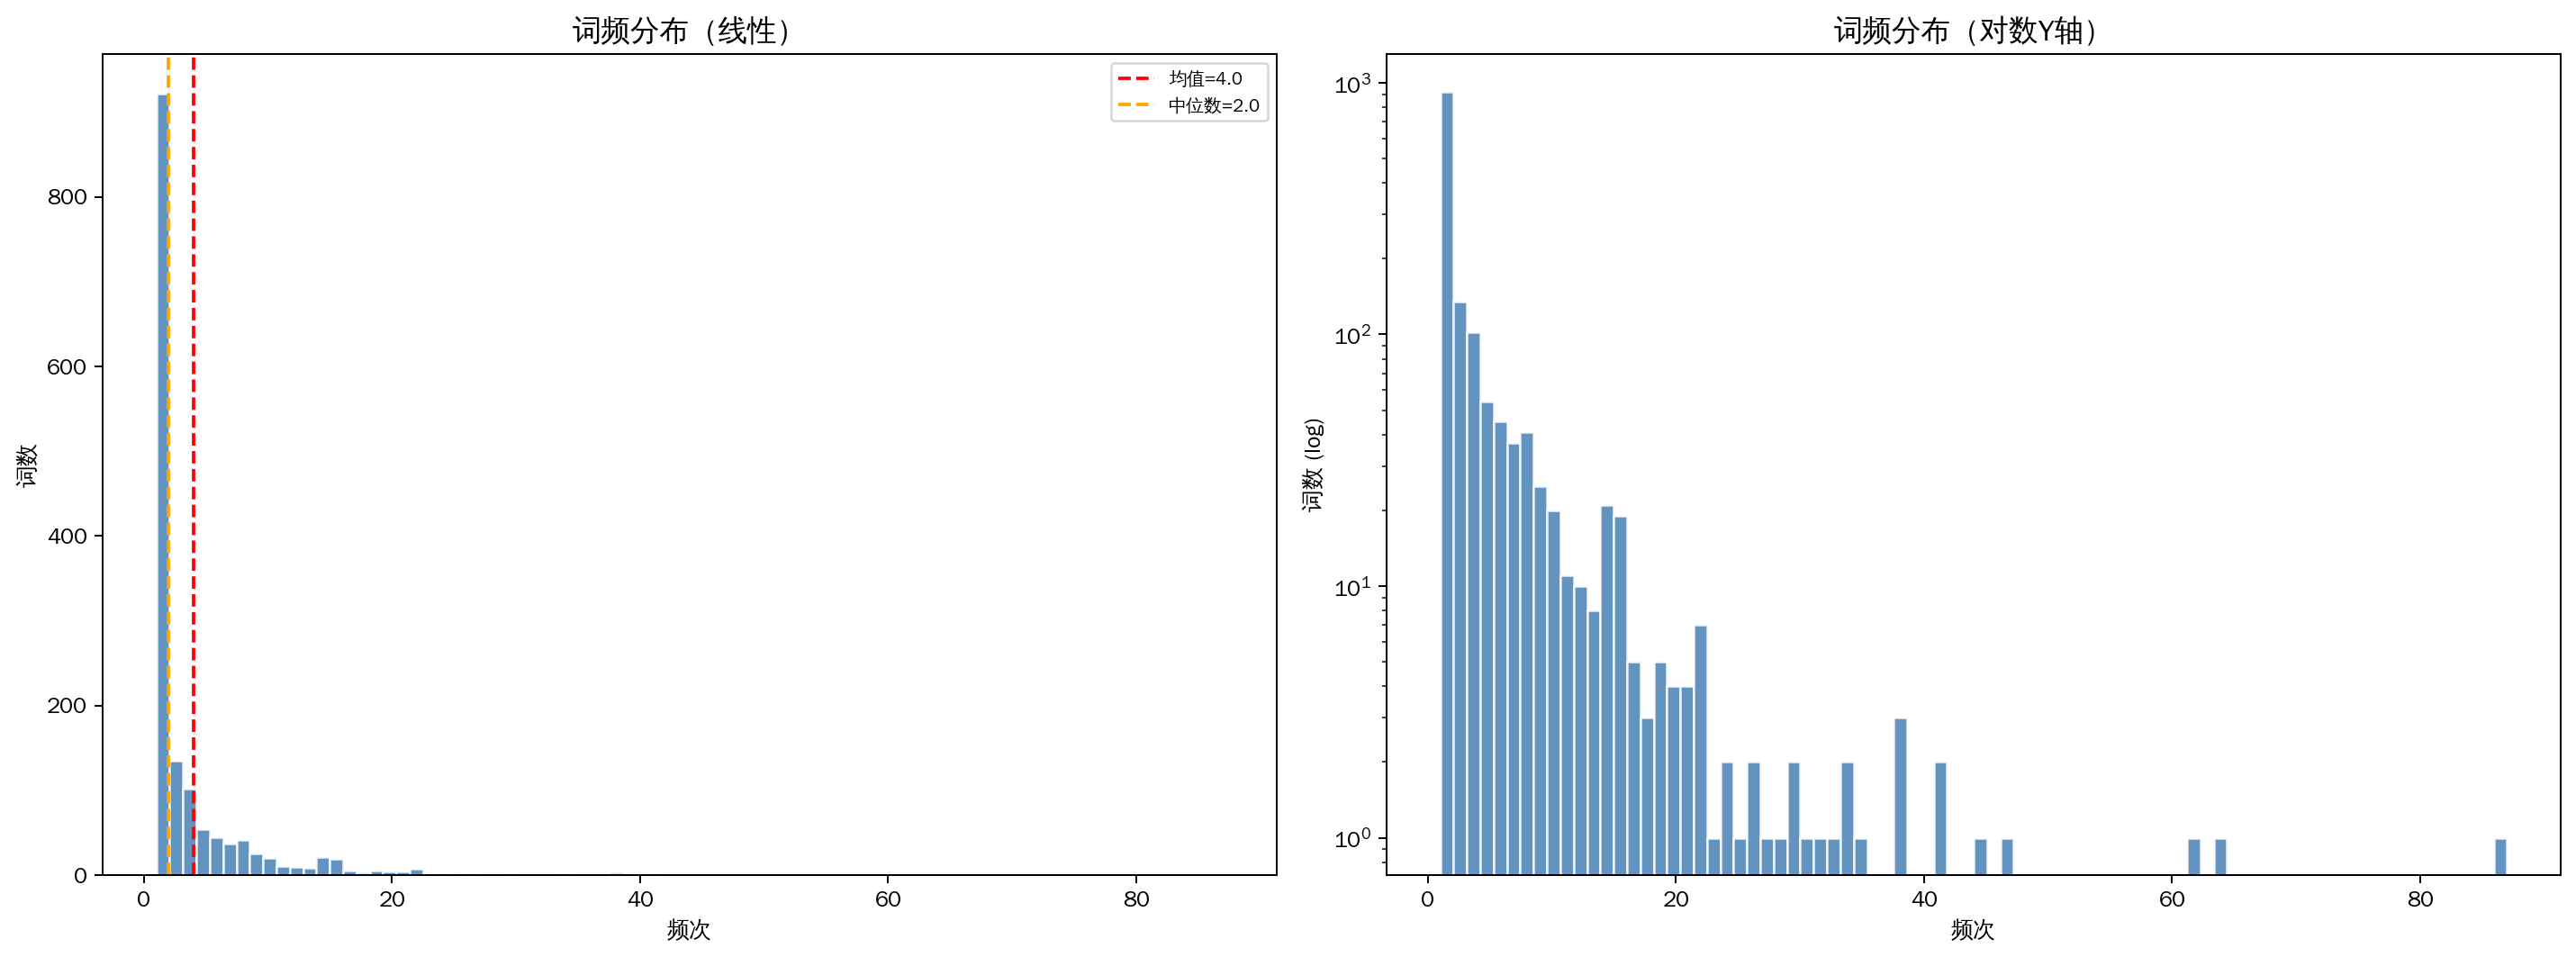
\includegraphics[width=0.95\textwidth]{figures/02_词频分布直方图.png}
\caption{词频分布直方图（左：线性 Y 轴；右：对数 Y 轴）}
\label{fig:hist}
\end{figure}

从线性坐标中可以清楚地看到，绝大多数词汇仅出现了 1 到 2 次，频次分布呈现出一条极为陡峭的下降长尾。在对数坐标下，低频词的分布跨度更加明显：出现过 1 次的词超过 1,200 个，占全部唯一词的约 65\%；出现 2 次的词约 170 个；出现 3 次以上的词数量急剧减少。这些仅出现一次的词中既包括 SKILL.md 等文档中出现的专业术语（如"滑窗""幂律""双对数"等仅在分析相关段落出现一次的名词），也包括代码中大量的一次性变量名和临时符号。低频词虽然占据了词表的主体，但它们在语料中的实际占用率极低；1,200 多个仅出现一次的词合计仅贡献了约 13.5\% 的总 token 量。这一比例关系反映了海量低频词在 token 层面微不足道的总权重，也意味着高频词的覆盖率分析将是理解语料集中度的更有效工具。

\subsection{Zipf 定律验证}

我们将去停用词后的词频按排名排列，在双对数坐标中绘制散点并做线性拟合，结果如图~\ref{fig:zipf} 所示。

\begin{figure}[htbp]
\centering
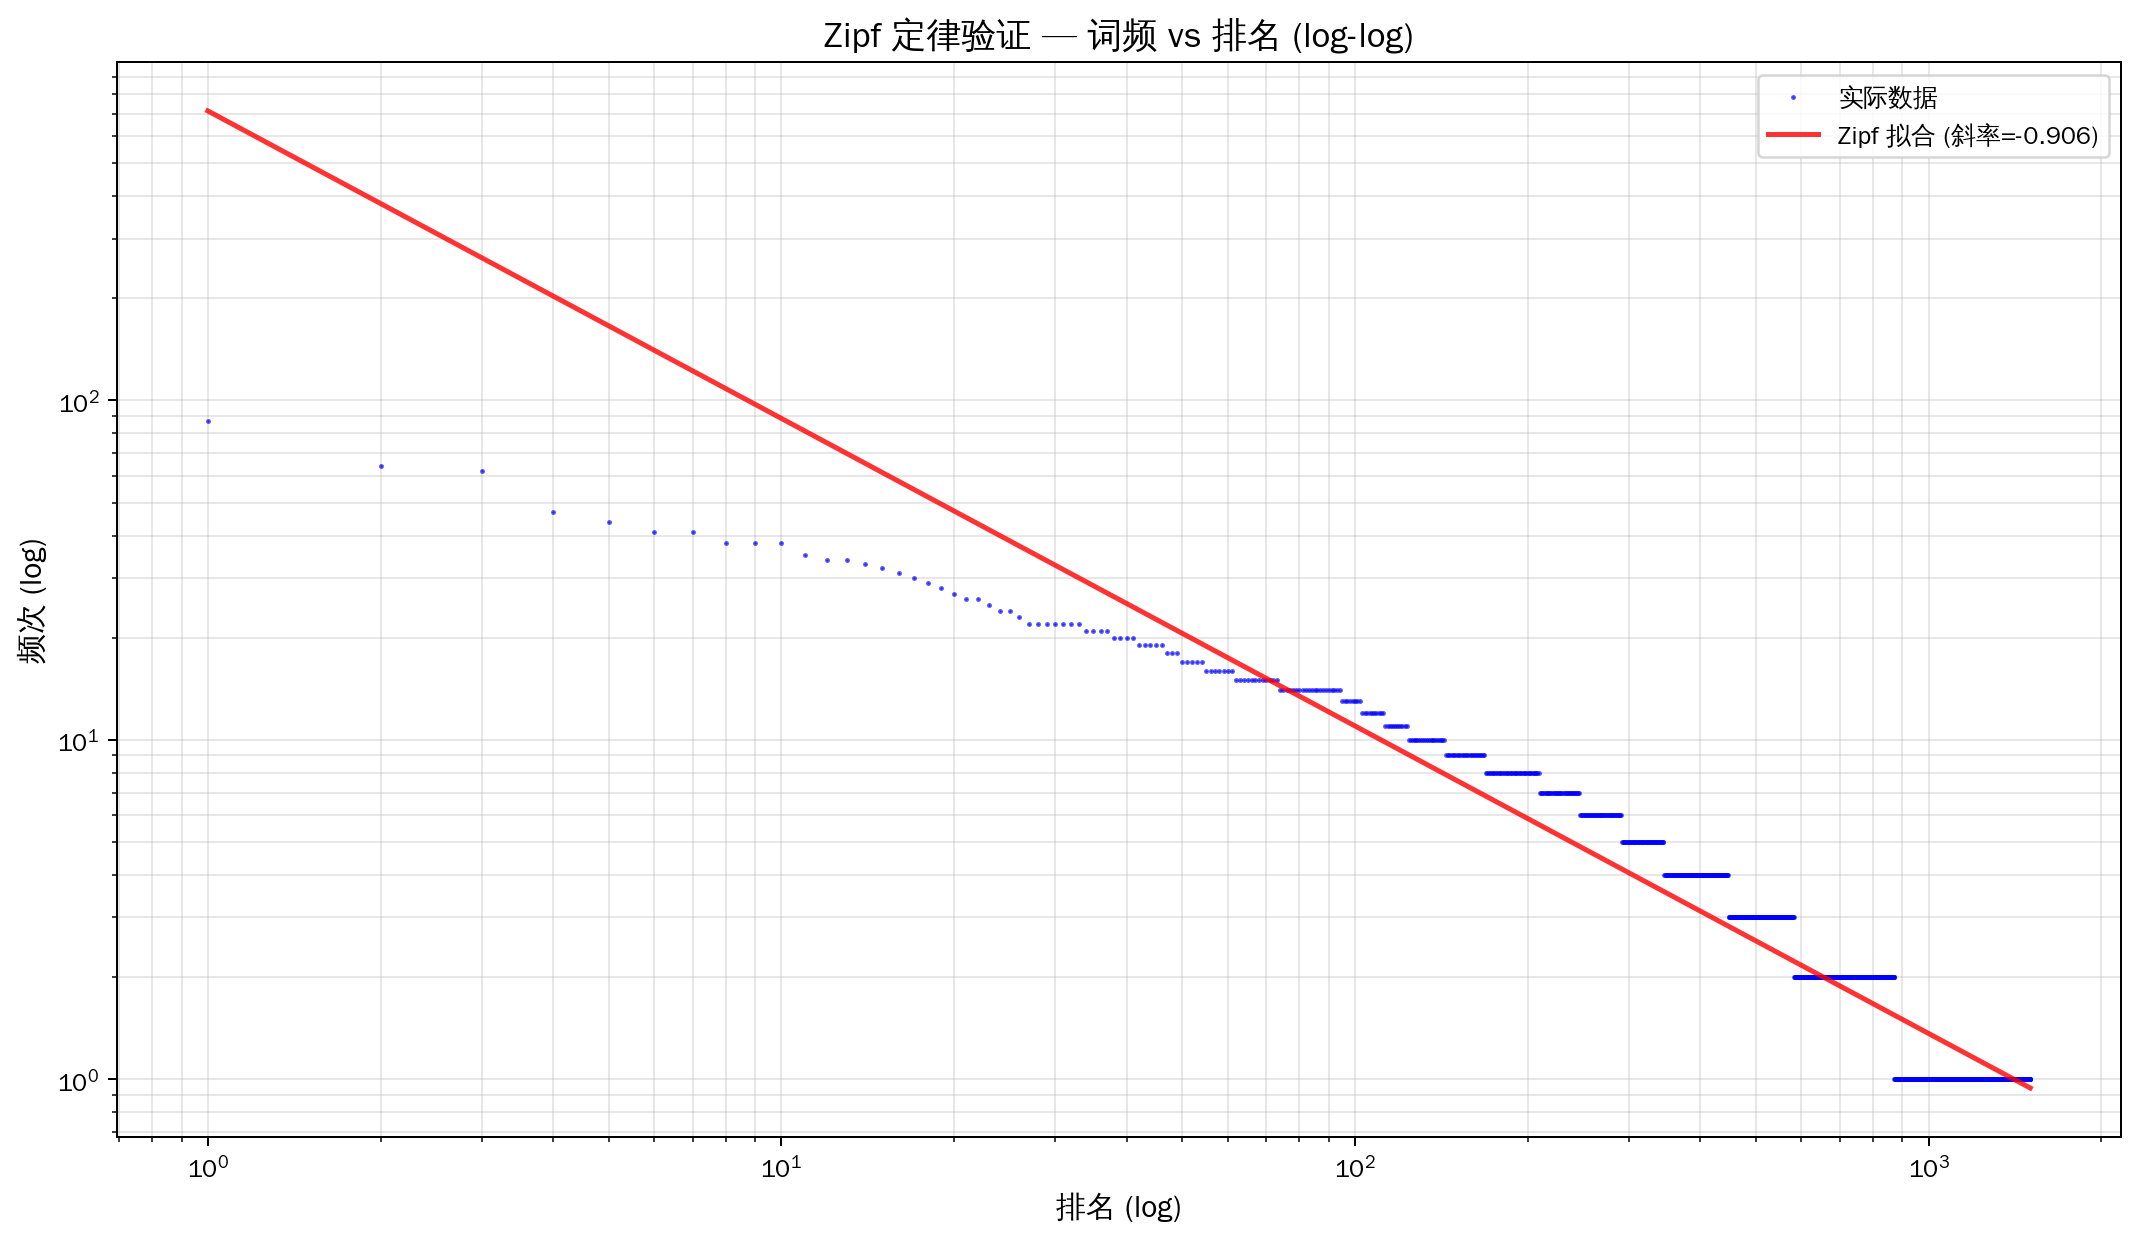
\includegraphics[width=0.85\textwidth]{figures/03_Zipf定律验证.png}
\caption{Zipf 定律验证：词频与排名在双对数坐标下的关系}
\label{fig:zipf}
\end{figure}

拟合得到的斜率为 \(-0.906\)，与理论值 \(-1.0\) 的偏差约为 9.4\%。在排名中段（约第 10 位到第 500 位），数据点紧密分布在拟合线两侧，表现为稳定的幂律行为。然而排名最高的前几个词（尤其是前两位的「实验」（87 次）和 ax（64 次））明显偏离拟合线，实际频次低于 Zipf 理论预期。这种"头部压低"现象需要放在该语料的具体构成中去理解。在典型的通用英语语料中，冠词 the 的频次往往远超介词 of，两者之间的频次差距可达数倍；这种巨大的差距使得在双对数坐标中前几位的下降斜率接近理论值。而在本语料中，「实验」87 次、「报告」62 次、「材料」47 次，这三个最高频词全部是内容词而非功能词，它们的频次受主题覆盖范围的约束，无法像功能词那样拉开巨大差距。与此同时，ax、print、len、set 等代码词汇以相近的频次（38--64 次）构成另一组高频词群，进一步拉平了前几十位的频次曲线。内容词群和代码词群在接近的频次区间内"挤"在一起，自然导致了头部的压低。

\subsection{累积覆盖率}

图~\ref{fig:cumulative} 展示了词频的累积覆盖率曲线，图中标注了 Top10、Top20、Top50、Top100 等不同截断点的累积覆盖比例。

\begin{figure}[htbp]
\centering
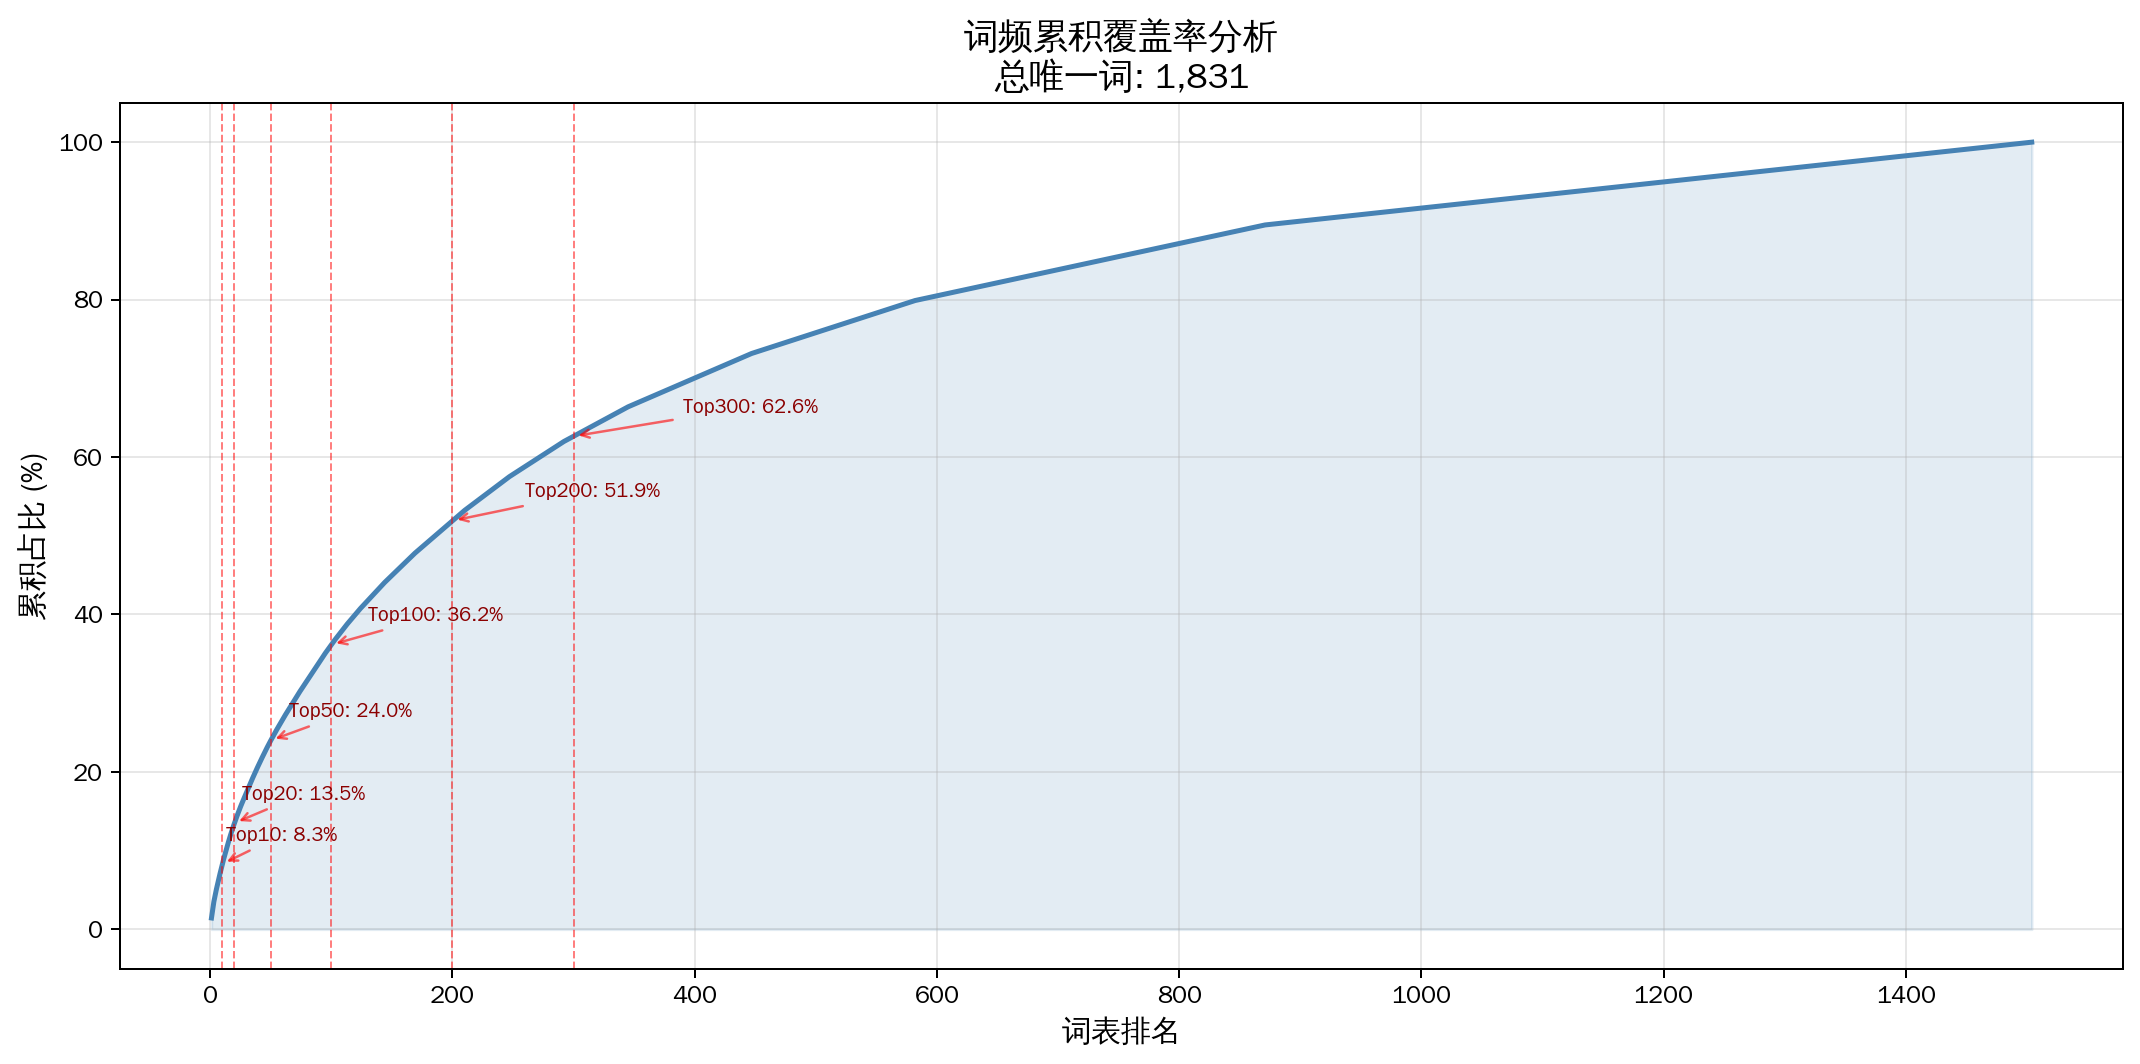
\includegraphics[width=0.88\textwidth]{figures/04_累积覆盖率.png}
\caption{词频累积覆盖率曲线}
\label{fig:cumulative}
\end{figure}

在全部 1,831 个唯一词中，前 10 个词覆盖了 8.3\% 的 token 总量，前 50 个词覆盖了 24.0\%，前 100 个词覆盖了 36.2\%。这意味着词表中约 5.5\% 的高频词（前 100 个）承担了超过三分之一的语料内容，而其余 94.5\% 的词分散承担了剩下的近三分之二。要达到 80\% 的累积覆盖率，需要约前 800 个词，接近整个词表的一半。在典型的大型通用语料中，前 100 个词通常可覆盖 45\%--55\% 的内容，本语料的 36.2\% 明显偏低。

造成覆盖率偏低的主要原因可以归结为高频词和低频词两个端点的共同作用。在高频端，语料的主题高度聚焦于"实验报告撰写"，此范围内的内容词数量有限；"实验""报告""材料""文件""教师""学生""内容""使用""检查""分析"等十个左右的词构成了高频段的核心，每个词的峰值不过 20--87 次，无法产生像通用语料中 the（动辄出现数万次）那样的绝对高频。在低频端，代码脚本贡献了大量仅出现一次的 token：Python 变量名、API 调用符号、临时捕获的路径名和函数参数，这些词在词表中存在但在各文件中互不重复，共同填充了分布的长尾。高频端"不够高"与低频端"太多"两个因素相互叠加，使得达到高覆盖率需要遍历更长的词表。

\subsection{N-gram 分析}

二元词组（bigram）和三元词组（trigram）的统计揭示了一个与词频分析互补的结构特征：在 N-gram 层面，代码 API 调用模式与自然语言搭配的频次几乎相当。表~\ref{tab:ngram} 列出了频次最高的前 5 个 bigram 和 trigram。

\begin{table}[htbp]
\centering
\caption{高频 Bigram 和 Trigram（前5位）}
\label{tab:ngram}
\begin{tabular}{@{}rll@{}}
\toprule
排名 & Bigram & 频次 \\
\midrule
1 & set \_ & 34 \\
2 & ax set & 27 \\
3 & 而 非 & 26 \\
4 & \_ dir & 24 \\
5 & \_ words & 23 \\
\midrule
排名 & Trigram & 频次 \\
\midrule
1 & ax set \_ & 27 \\
2 & out \_ dir & 19 \\
3 & tf \_ idf & 16 \\
4 & most \_ common & 14 \\
5 & cum \_ pcts & 14 \\
\bottomrule
\end{tabular}
\end{table}

Bigram 的前两项——set \_（34 次）和 ax set（27 次）——来自 matplotlib 中 \texttt{ax.set\_title()}、\texttt{ax.set\_xlabel()} 等绘图 API 的调用模式。值得注意的是，"而 非"以 26 次排在第三位，与代码 bigram 的频次相当。这个中文搭配主要来源于 SKILL.md 中对措辞约束的反复强调——"而非罗列""而非隐藏"等表述多次出现。代码 N-gram 和自然语言 N-gram 在相近的频次区间中并排出现，意味着在 bigram 层面，代码片段的话语量级并不低于自然语言部分。Trigram 的前五名更是几乎全部来自代码模式：ax set \_ 对应绘图 API 的三 token 调用链，tf \_ idf 和 cum \_ pcts 分别对应 TF-IDF 计算和累积覆盖率计算的变量名，most \_ common 则是 Counter 对象的常用方法调用。

这种代码 N-gram 占主导的现象并不是分词或统计的失误，而是我们语料构成的直接体现。分析脚本中的 Python 代码在被分词后形成了一个密集的短 token 序列，每个方法调用、变量赋值和循环体中的符号都成为 N-gram 滑窗的输入。在一个 8 个文件的小语料中，一份 1,721 token 的脚本足以在 N-gram 层面占有与自然语言文档同等的比重。图~\ref{fig:bigram} 展示了 Bigram Top20 的完整分布——前二十项中代码相关模式占据了约三分之二。

\begin{figure}[htbp]
\centering
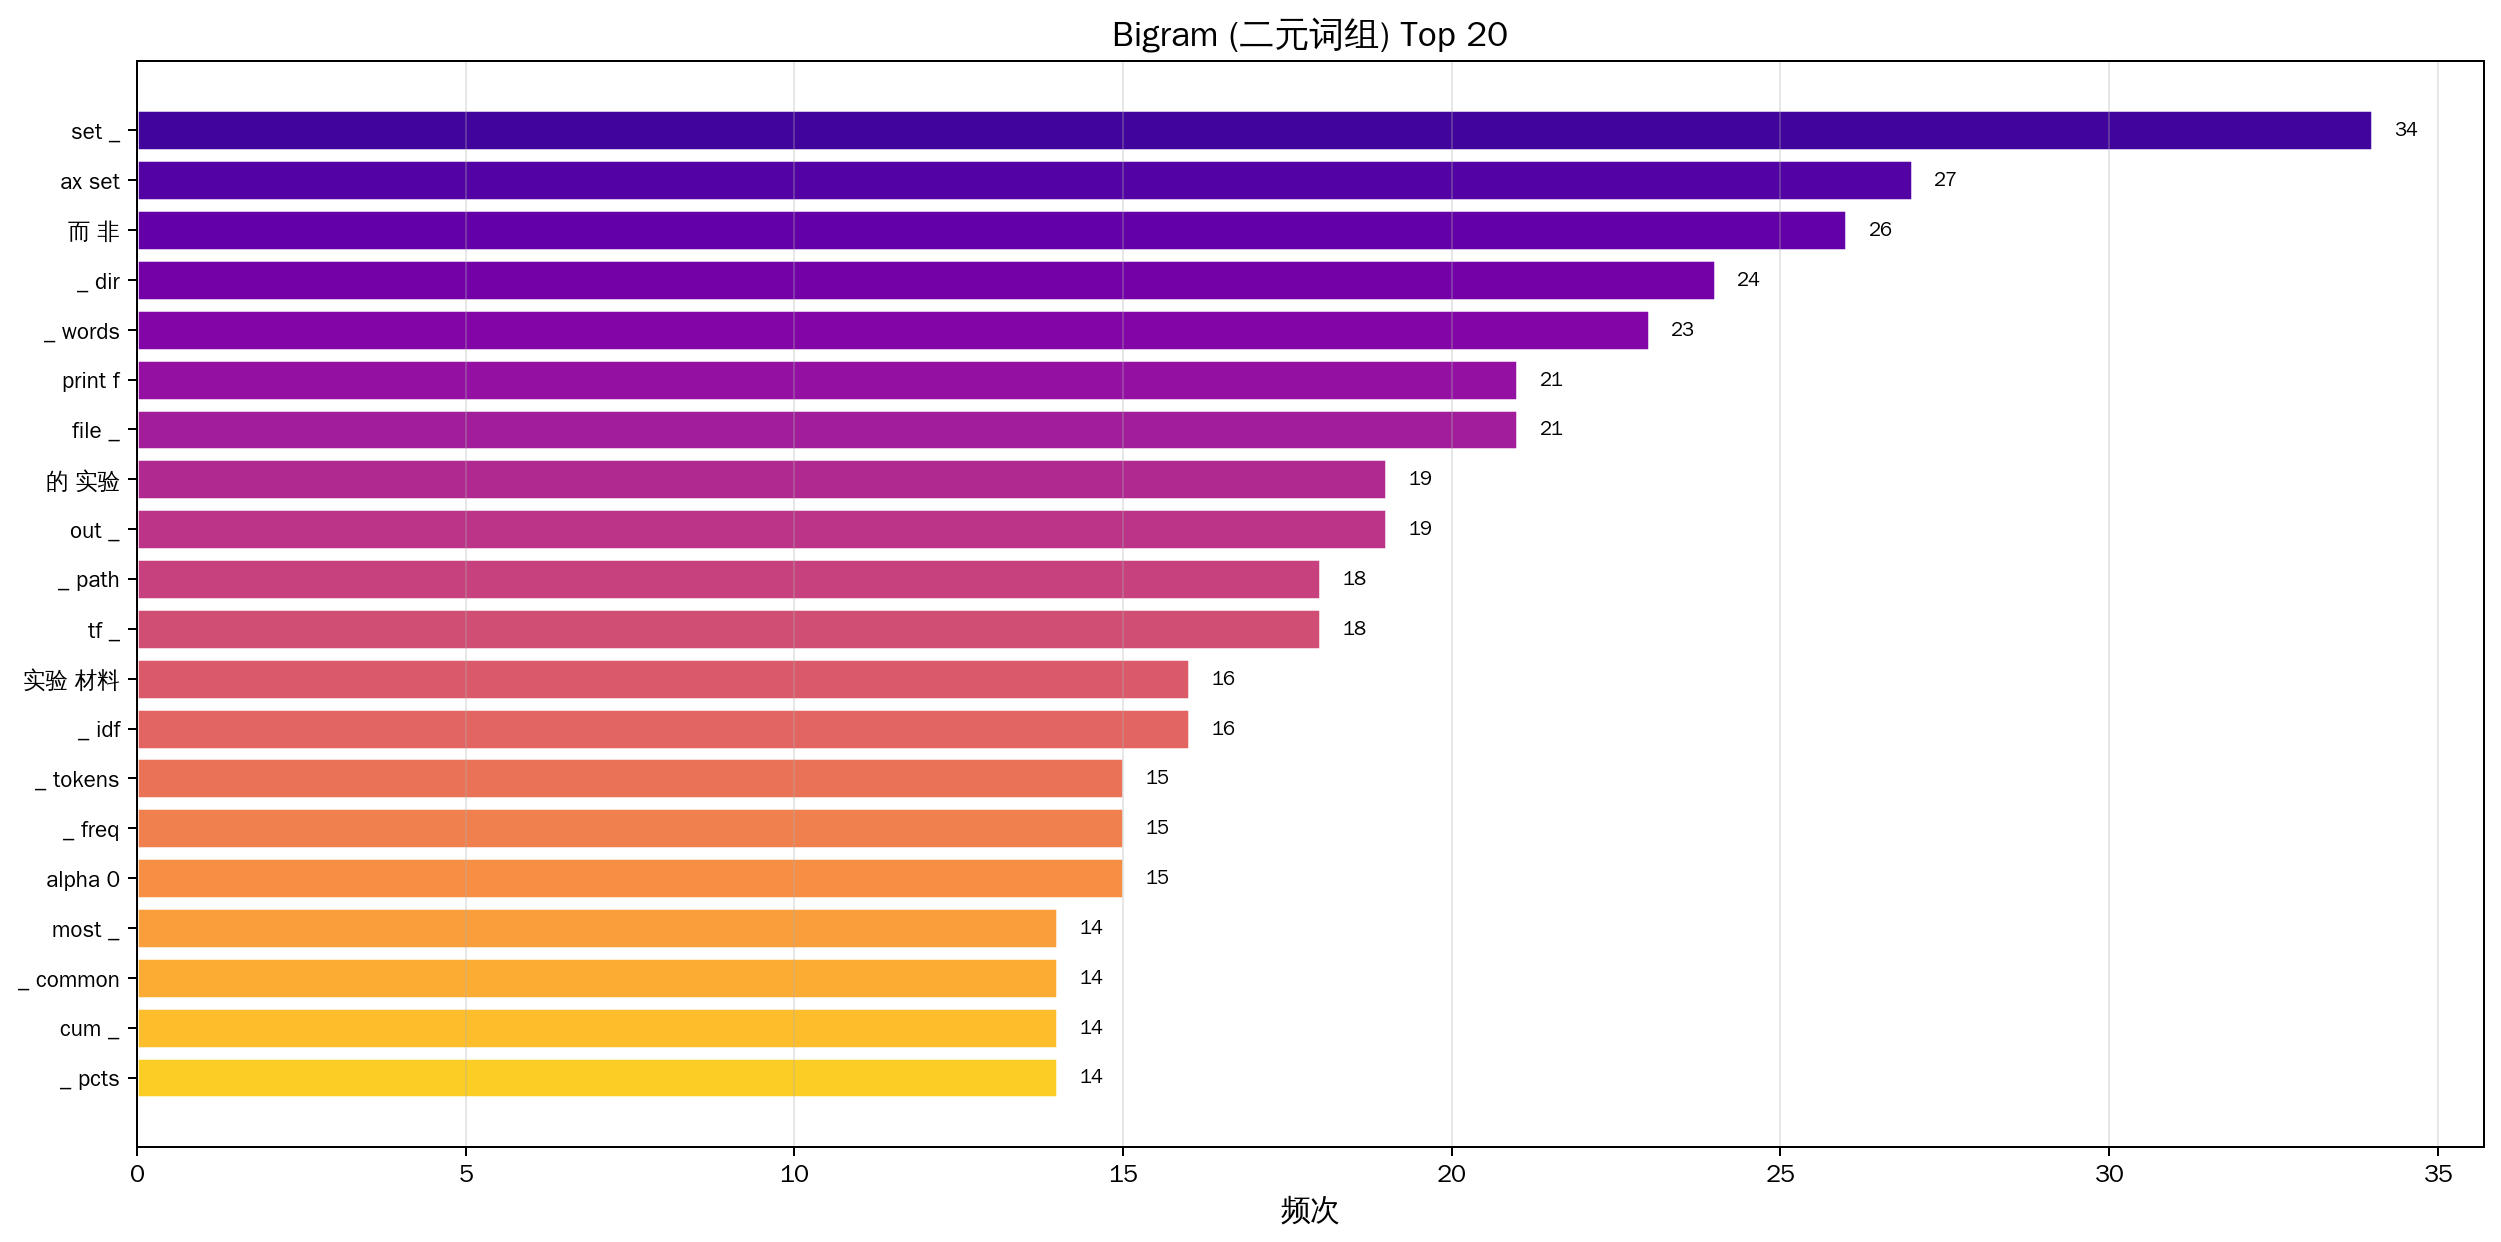
\includegraphics[width=0.88\textwidth]{figures/05_Bigram_Top20.png}
\caption{Bigram 词组频率 Top 20}
\label{fig:bigram}
\end{figure}

\subsection{TF-IDF 关键词提取}

TF-IDF 分析从文件区分度的角度提供了另一种视角。表~\ref{tab:tfidf} 列出了得分最高的前 10 个关键词。

\begin{table}[htbp]
\centering
\caption{TF-IDF 关键词 Top 10}
\label{tab:tfidf}
\begin{tabular}{@{}rrr@{}}
\toprule
排名 & 词汇 & TF-IDF 得分 \\
\midrule
1 & \_ (下划线) & 0.0841 \\
2 & experimental & 0.0489 \\
3 & path & 0.0388 \\
4 & report & 0.0384 \\
5 & experiment & 0.0366 \\
6 & course & 0.0326 \\
7 & ready & 0.0326 \\
8 & materials & 0.0326 \\
9 & 该 & 0.0279 \\
10 & ax & 0.0273 \\
\bottomrule
\end{tabular}
\end{table}

一个显著但容易忽视的结果是：TF-IDF 得分最高的词是下划线符号 \_，得分为 0.0841，远超第二名 experimental（0.0489）。下划线作为 Python 中常见的临时变量名占位符，在分析脚本中频繁出现，而在其他 Markdown 文档中几乎不出现。它在数学上完美符合 TF-IDF 的"文件标志词"定义——在某文档内高频、在全局语料中稀有——但作为一个无语义的语法符号，它的高分恰恰暴露了 TF-IDF 在代码与自然语言混合语料中的一个系统性问题：TF-IDF 不区分"有语义的关键词"和"无语义的语法符号"，后者只要分布足够不均匀，就能获得高得分。

experimental、report、experiment、course、materials 等英文词以相近的得分（0.0326--0.0489）聚集在第二梯队。这一组词的高分来自 README.md——该文件是 8 个文件中唯一大量使用英文叙述的文档，而这些词在其他中文为主的文档中几乎不出现，因而其逆文档频率接近理论最大值。值得注意的是，course、ready、materials 三个词的得分完全相同（0.0326），这是因为它们在 README.md 中频次相近，且在其他 7 个文件中均不出现在去停用词后的有效词表中，导致三者的 IDF 值完全一致——这是小语料分析中一个精确定量但未必有区分意义的巧合。图~\ref{fig:tfidf} 展示了 TF-IDF 得分 Top20 的完整分布。

\begin{figure}[htbp]
\centering
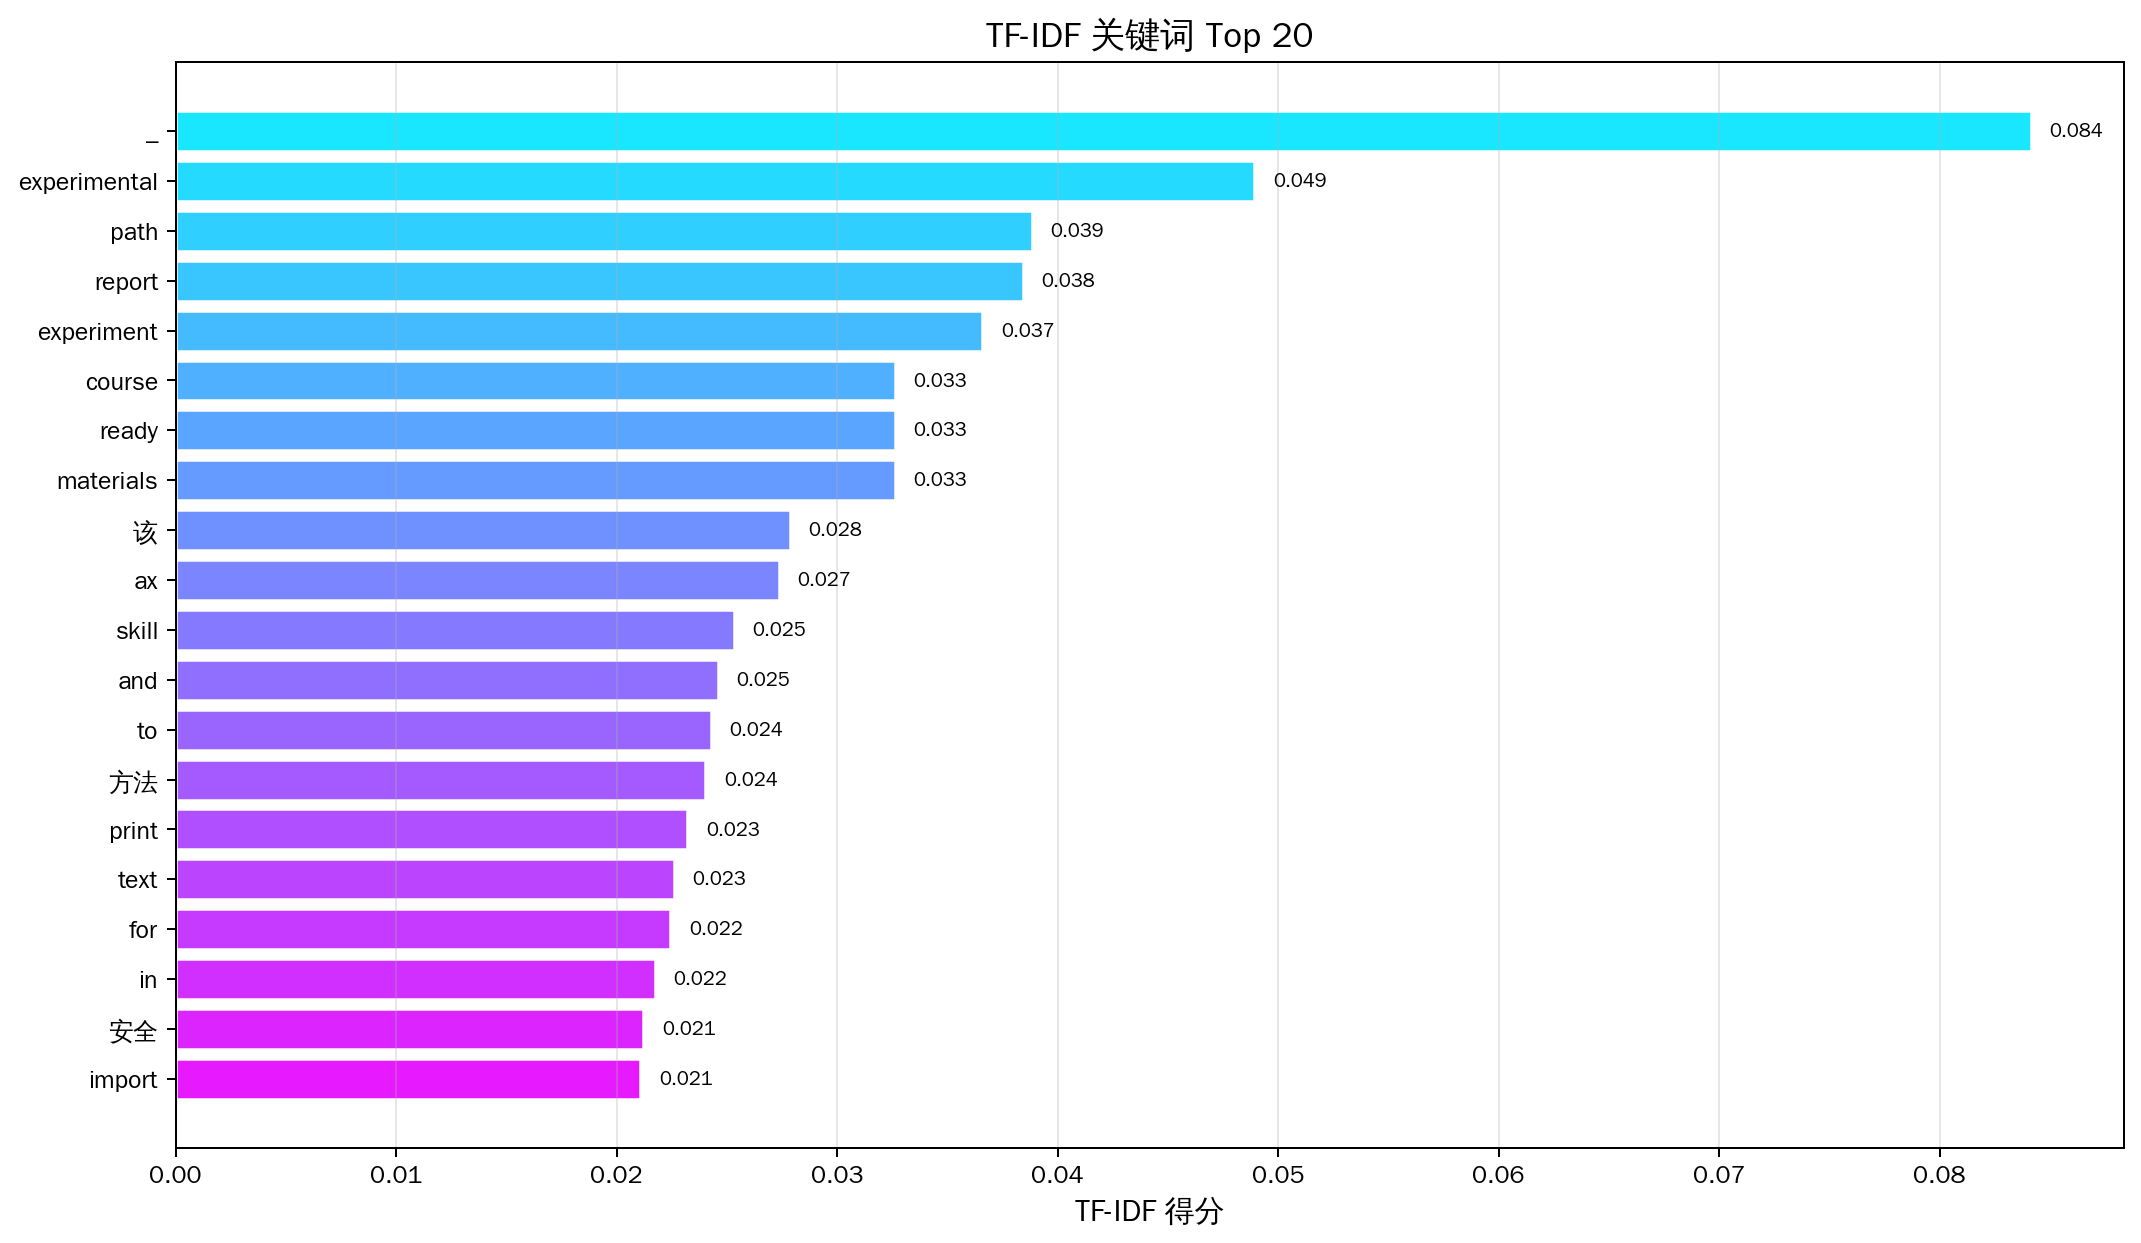
\includegraphics[width=0.82\textwidth]{figures/09_TF-IDF_Top20.png}
\caption{TF-IDF 得分 Top 20}
\label{fig:tfidf}
\end{figure}

\subsection{文件间词频对比}

我们对不同文件中的高频词分布做了归一化处理，得到了如图~\ref{fig:heatmap} 所示的热力图。每个文件构成一列，全局 Top20 高频词中的每一个构成一行，颜色深浅反映该词在该文件中的归一化频率。

\begin{figure}[htbp]
\centering
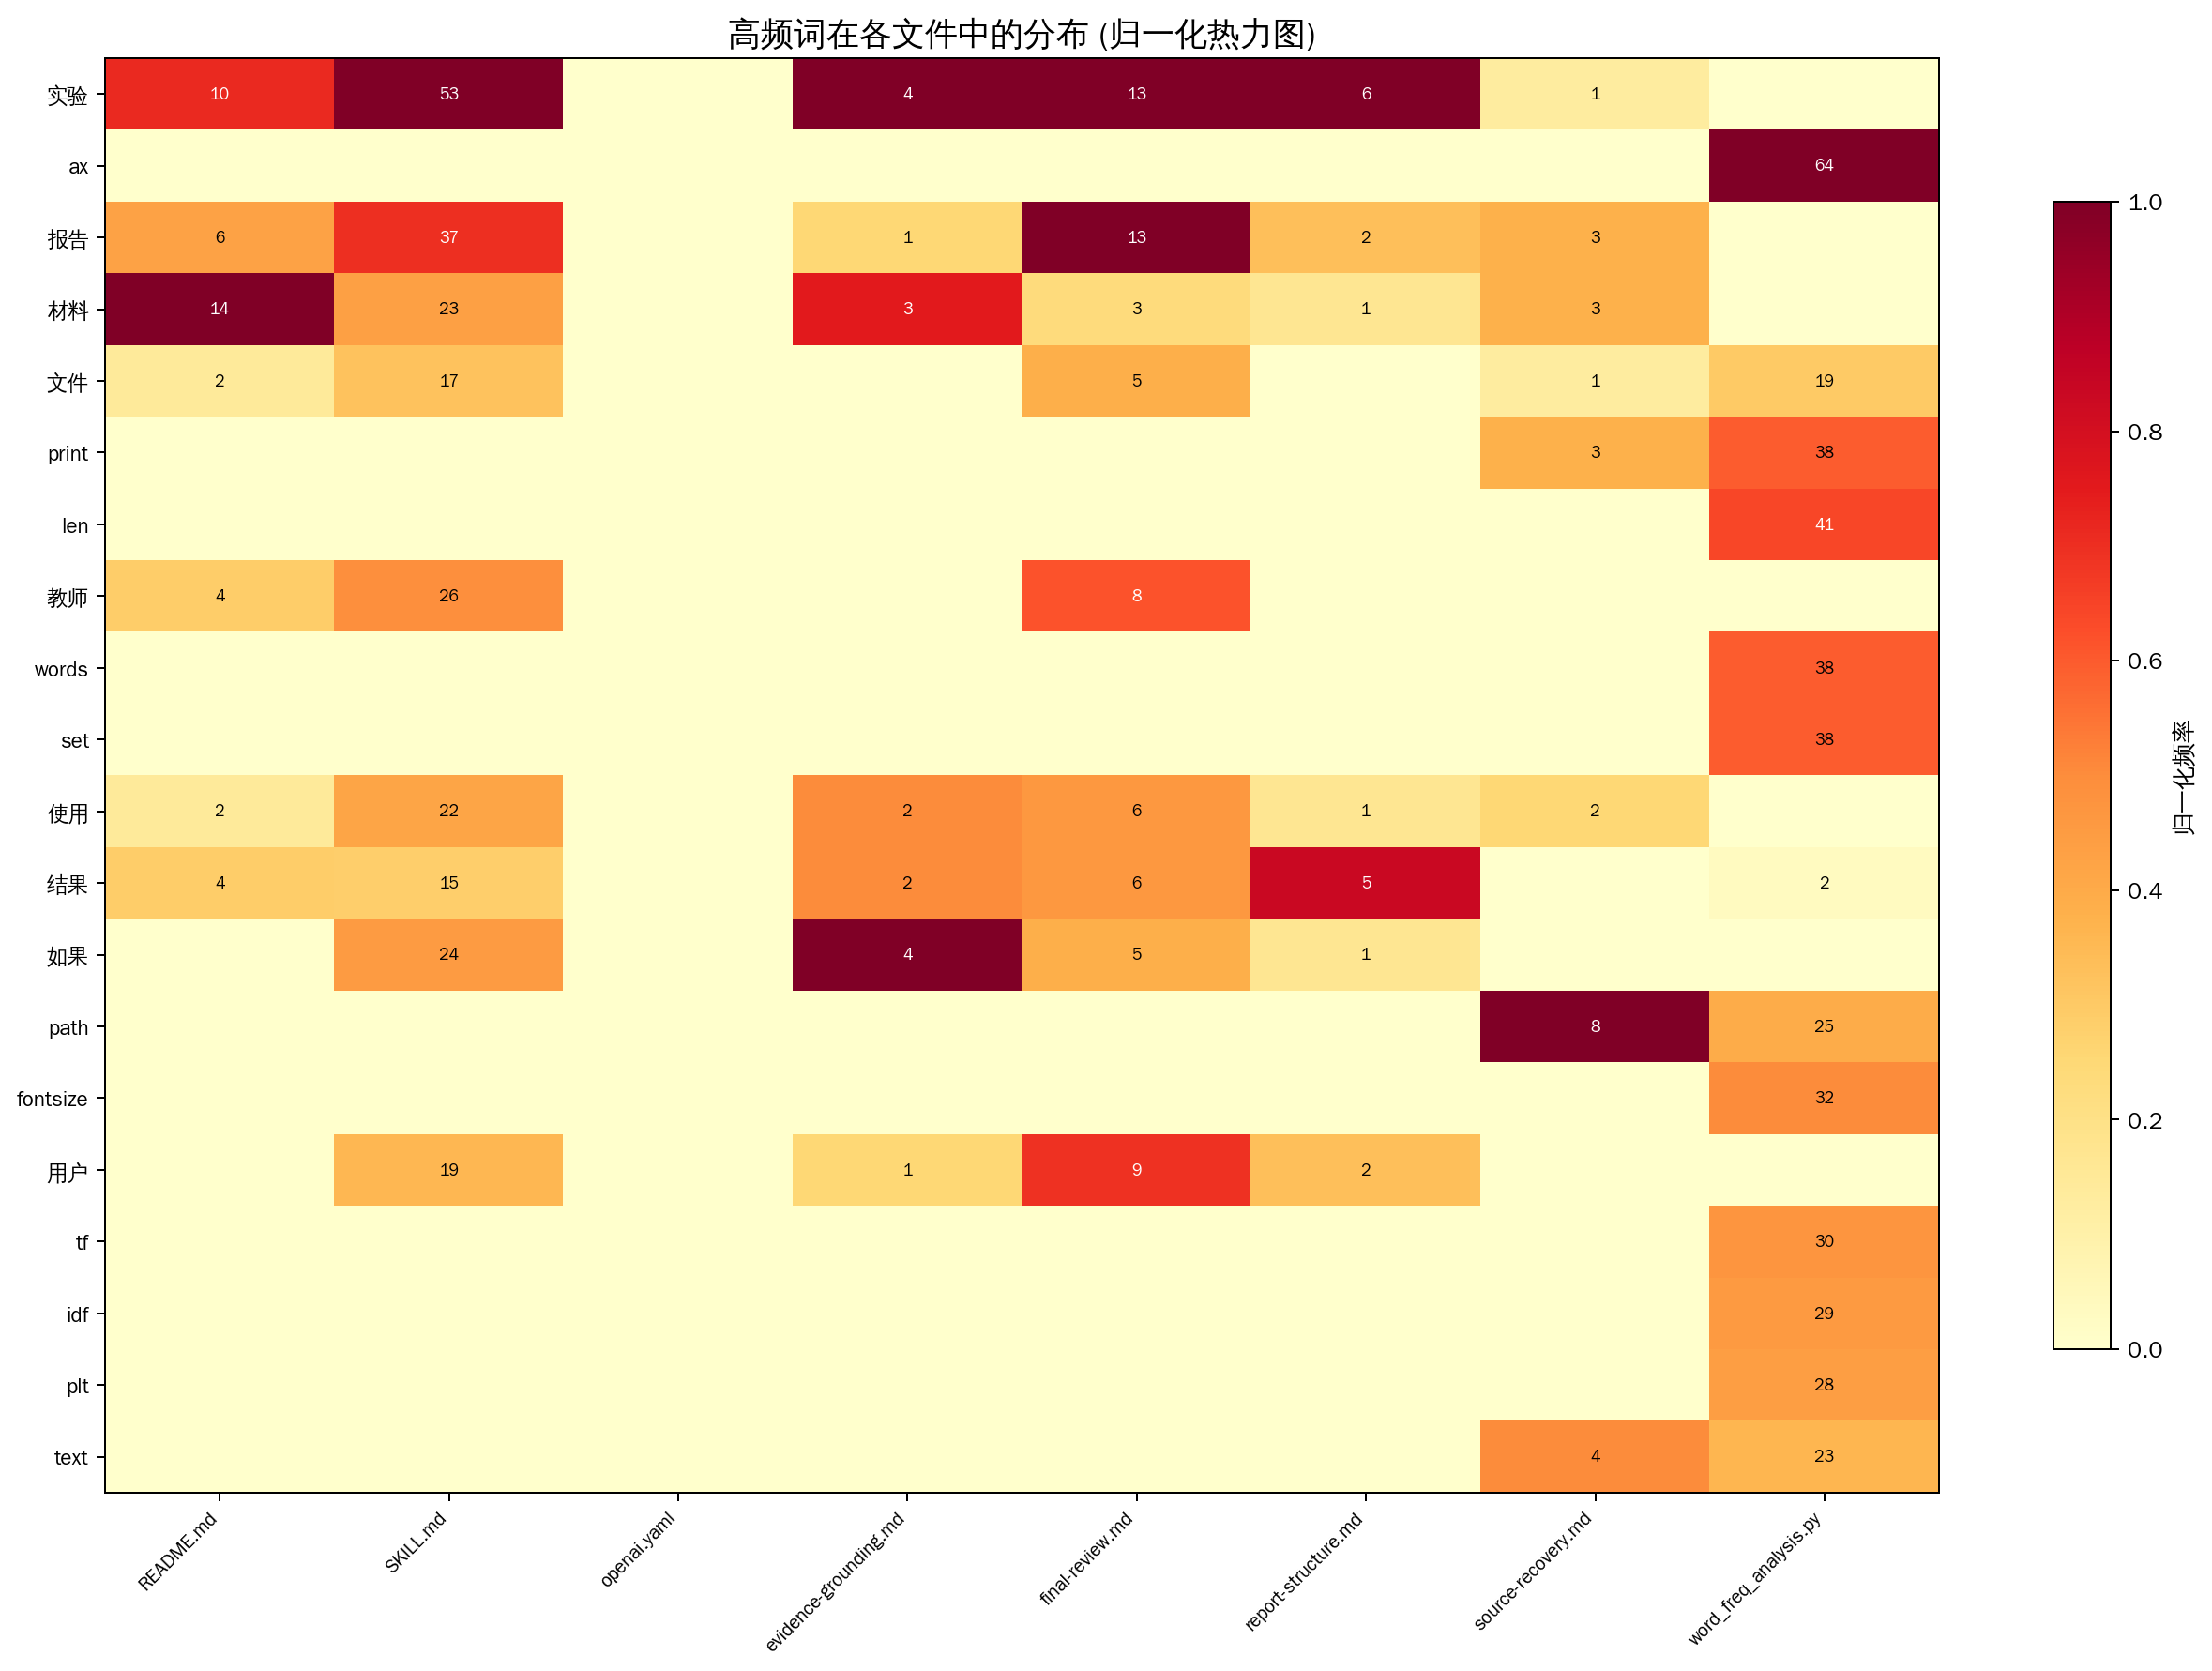
\includegraphics[width=0.92\textwidth]{figures/07_文件间词频热力图.png}
\caption{全局高频词在各文件中的分布（归一化热力图）}
\label{fig:heatmap}
\end{figure}

热力图揭示了文件之间的三种分化模式。第一类是 SKILL.md，它几乎在所有全局高频词上都有显著贡献，颜色在大多数行上均匀较深。原因在于它的篇幅和覆盖面——8,390 字符的长度使其远超其他文件，且内容遍历了实验报告的全流程，因此高频主题词在其词表中全面出现。第二类是 README.md，其色块集中在 experimental、report、course 等英文关键词所在的行——该文件以英文摘要方式描述技能功能，极少涉及「实验」「材料」「教师」等中文主题词，因而在那些行上几乎无色。第三类是 word\_freq\_analysis.py，它对 print、len、words、set 等 Python 技术词贡献最大，在这些行上颜色极深；而在中文主题词行上则几乎不出现，因为脚本的 docstring 中虽包含中文注释，但其 token 量相较于代码部分比例很小。这种文件间的功能分化——叙述全面型（SKILL.md）、英文摘要型（README.md）和技术实现型（脚本）——在一张 8 列的归一化热力图上得到了精确且易于阅读的呈现。

\subsection{词云可视化}

为提供对语料整体面貌的直观感知，我们基于去停用词后的词频生成了词云，如图~\ref{fig:wordcloud} 所示。词云中字体大小与词汇频次成正比。

\begin{figure}[htbp]
\centering
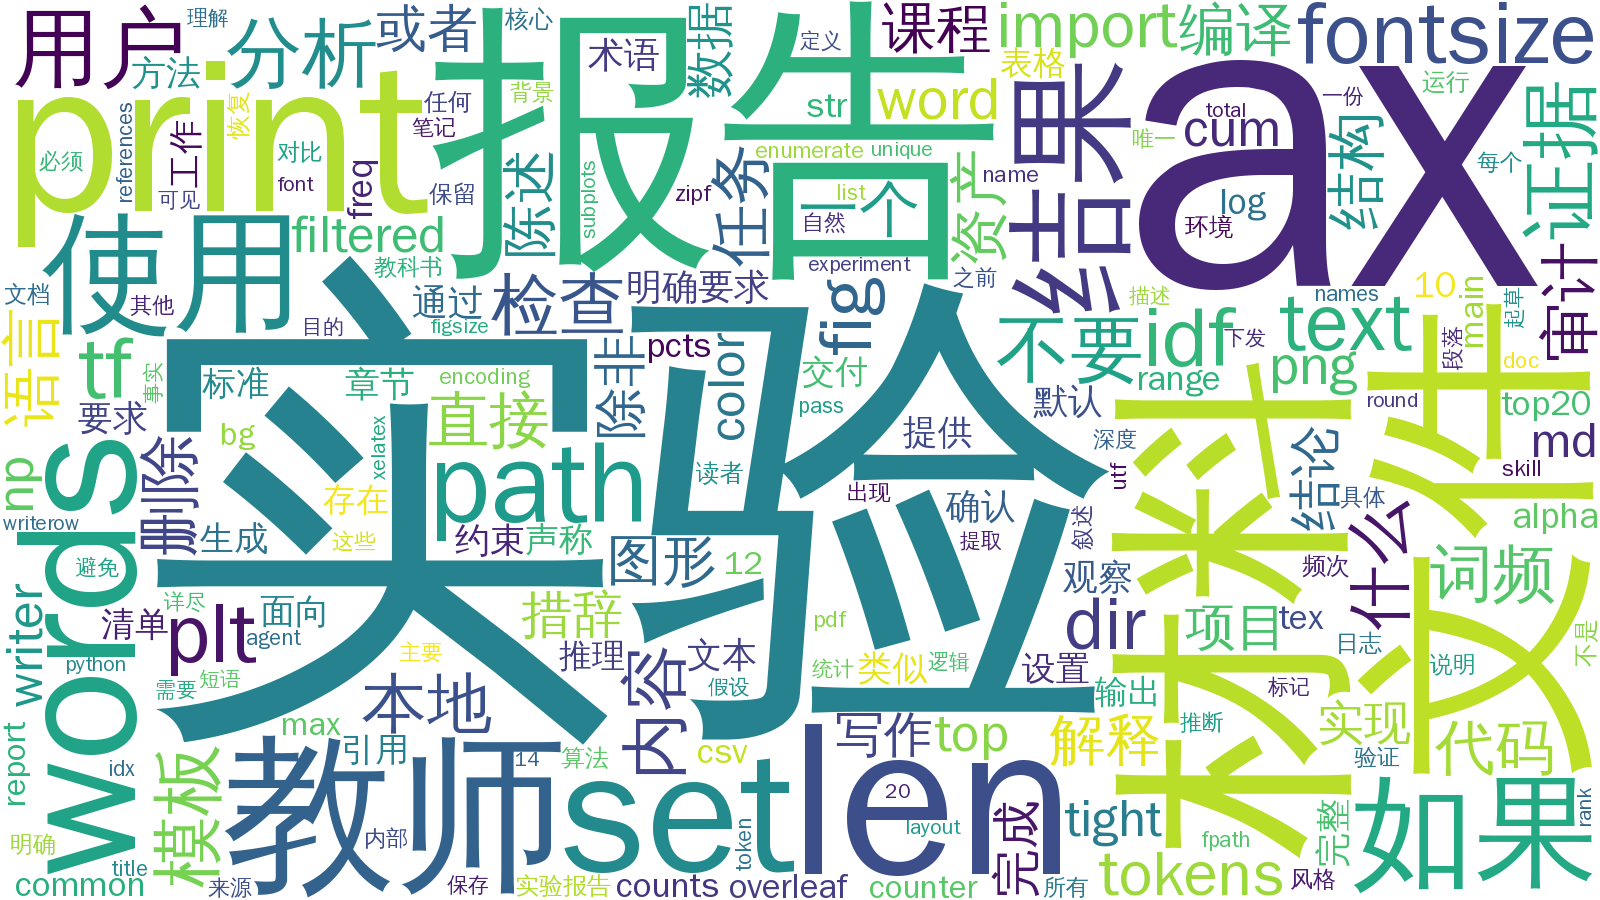
\includegraphics[width=0.88\textwidth]{figures/06_词云.png}
\caption{词频词云}
\label{fig:wordcloud}
\end{figure}

占据视觉中心的词——「实验」「材料」「教师」「文件」「使用」——以大号字体直接确证了语料围绕课程实验报告的主题定位。英文技术词汇如 print、set、len、path、text 等散布在词云的各个方向，其字号与部分中文主题词汇相当，这意味着在可视化层面代码相关词汇的视觉权重与主题词汇处于同一级别。在词云生成过程中，我们使用了文泉驿正黑作为中文字体——若使用默认的 DejaVu Sans，所有中文字符将显示为方框，只有英文部分可见，词云将完全失去对中文语料的描述能力。

\section{结果分析}

\subsection{词表构成的混合特征}

词频 Top30 和 N-gram Top20 的结果共同指向一个结构特征：中文主题词与 Python 代码关键词在频次上处于同一量级，代码片段对语料统计的影响力容易被低估。脚本仅占文件数量的 1/8，但贡献了 19.4\% 的有效 token 量，原因不仅是它本身的长度，更在于代码 token 的产生密度——自然语言中大量的虚词、标点经过停用词过滤后不再计入统计，而代码中的每一个变量名、符号和函数调用都被保留为有效 token，使得脚本在有效词频统计中的相对权重被系统性放大。

在 N-gram 层面，ax set（27 次）和「而 非」（26 次）的频次几乎相等，但两者的语义性质截然不同。我们追踪了 ax set 的生成路径：在原始代码中 \texttt{ax.set\_title()} 是一个完整的语义单元，但 jieba 按点号（\texttt{.}）和下划线（\texttt{\_}）边界将其切分为 ax、set、\_ 和 title 四个独立 token，bigram 滑窗再将相邻的 ax 与 set 重新组合为 ax set 这一词组。而「而 非」是一个连贯的中文搭配，在分词后保持了语义完整性。两种 N-gram 在频次上等价，但在信息上有质的差异——一种是有意义的转折连接词，另一种是 API 调用模式的 token 碎片。在全量统计中不对两者做区分是诚实的，但在解读结果时需要对这种质的差异保持清晰的认识。

\subsection{Zipf 拟合斜率偏离的多因素解释}

拟合斜率为 \(-0.906\)，偏差方向为"负得不够"——即实际词频下降得比 Zipf 定律预测的要慢。这意味着高频词之间的差距比理论预期小，中低频词的频次比理论预期高。我们从两个方向来理解这个偏离。

首先，语料的主题高度聚焦。在通用语料中，排位第一的功能词（如 the）通常远超排在第二的功能词（如 of），两者之间的频次差距巨大，使得头部下降非常陡峭。而在本语料中，排位第一的「实验」87 次，第二的 ax 64 次，两者之间的倍数仅为 1.36。排位第一到第十的频次从 87 缓慢下降到 38——如果将这些词按频次画成一个数列，下降的坡度远低于通用语料中的前十个词。原因是这些词都是内容词（而非功能词），它们的频次共同受限于语料的总规模和主题覆盖范围，同一主题内的内容词本身就会发生频次上的"粘连"，无法像功能词那样拉开层级差距。

其次，代码词群在 Top10--Top30 区间形成一个额外的频次平台。print、len、set、words、text、path 等词在 20--41 次区间密集出现，它们与自然语言的中高频词（使用、结果、如果等）混合排列，使得排名曲线的中段下降进一步放缓。代码 token 的相对均匀分布——因为脚本中的常用 API 调用模式都出现了若干次——对排名频次曲线起到了一种"削峰填谷"的作用。

\subsection{覆盖率偏低的结构原因}

累积覆盖率 36.2\%（Top100）在通用语料中偏低，但从本语料的构成来看是一个合理的结果。我们把覆盖率分解为两个来源的贡献来衡量。高频端：前 10 个词合计贡献了约 740 个 token，占总 token 的 8.3\%。这些词的主体是中文主题词和代码高频词，每个词的平均贡献约 74 个 token——这个绝对值不高，因为语料总规模只有 8,882 个 token，单个主题词不可能出现成百上千次。低频端：超过 1,200 个仅出现一次的词合计贡献了约 1,200 个 token，占总 token 的 13.5\%——这个比例正好说明，大量的唯一 token 虽然占词表的 65\%，但对总内容的贡献并不大。真正拉低覆盖率的不是这些仅出现一次的词，而是分布在第 100 位到第 800 位之间的中频词群——它们数量众多（约 700 个），每个词出现 2--4 次，合计覆盖了约 40\% 的总 token。这个中频"高原"是覆盖率曲线缓慢爬升的直接原因，而这些中频词主要来自代码中的重复但非极高频率的模式（如不同的路径名、不同的参数名、不同的 Markdown 章节标题等）。

\section{结论}

我们通过本次实验对 8 个文本文件实施了系统的词频统计分析，建立了覆盖词频、N-gram 词组频率、TF-IDF 关键词和 Zipf 定律验证的多维度分析框架。

该语料的词频分布在整体上服从 Zipf 定律的幂律衰减——拟合斜率 \(-0.906\)，中段数据表现稳定——但最高频词受语料主题集中度和内容词特性影响，出现了明显的头部压低。累积覆盖率分析表明，前 100 个高频词覆盖了语料 36.2\% 的内容，这一集中度在同等规模的主题语料中处于合理范围；覆盖率偏低的主要原因是内容词高频差异小和代码 token 的中频填充效应共同作用的结果。

语料的内部结构呈现出三种功能分化的文件组别：SKILL.md 作为覆盖面最广的文档在所有主题词上贡献最大，README.md 在中英文模式上与前者形成互补，而分析脚本自身则以差异化的技术词汇贡献构成了独立的分组。N-gram 分析揭示了一个方法层面的重要事实：代码 API 调用模式在 token 化后产生的 N-gram 在频次上与自然语言搭配相当——ax set 和「而 非」同为约 27 次——这要求分析者在解读结果时对代码来源的 N-gram 和自然语言来源的 N-gram 在语义上进行质的区分。

我们建立的文本分析流水线——jieba 分词、Counter 统计、N-gram 提取、TF-IDF 计算、matplotlib 可视化和 Zipf 验证——不依赖外部 API 或大型预训练模型，仅使用 Python 标准库和少量第三方包即可完成从原始文本到多维统计图表的全流程分析。该流水线在本次实验的小规模中英混合语料上表现出了预期的分析能力，对词频分布中的结构特征、异常点和文件间差异均给出了可核查的解读。

\end{document}
